\documentclass{standalone}
\usepackage{tikz}
\usepackage{ctex,siunitx}
\usepackage{tkz-euclide}
\usepackage{amsmath}
\usetikzlibrary{patterns, calc}
\usetikzlibrary {decorations.pathmorphing, decorations.pathreplacing, decorations.shapes,}
\begin{document}
\small
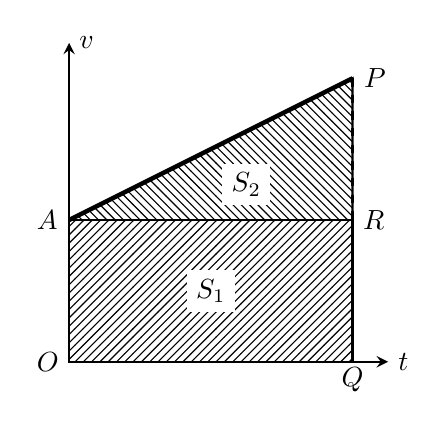
\begin{tikzpicture}[>=stealth, thick,scale=0.9]
  \draw [<->](0,4.5)node [right]{$v$}--(0,0)node [left]{$O$}--(4.5,0)node [right]{$t$};
  \draw [ultra thick] (0,2)node [left]{$A$}--(4,4)node [right]{$P$};
  \draw [dashed](4,4)--(4,0);
  \fill [pattern = north east lines, draw] (0, 0) rectangle (4, 2);
  \fill [pattern = north west lines, draw] (4, 2)-- (4, 4)--(0,2);
  \node at (4,-.25){$Q$};
  \node at (2,1)[fill=white]{$S_1$}; 
  \node at (4.3,2){$R$}; 
  \node at (2.5,2.5)[fill=white]{$S_2$};
\end{tikzpicture}
\end{document}